\chapter{Embeddings}

\epigraph{
    Nets are for fish; once you get the fish you can forget the net.\\
    Words are for meaning; once you get the meaning you can forget the words.
}{Zhuangzi}

\newpage

\section{Introduzione}
Quando leggiamo un testo, noi esseri umani siamo dotati della capacità di coglierne un aspetto di significato. Questo implica che dietro alle parole che leggiamo si cela una rappresentazione semantica che vorremmo potenzialmente far apprendere anche alle macchine.  
Dal momento che le macchine parlano con la lingua dei numeri e, non come noi, con quella delle parole è stato necessario introdurre degli strumenti che vorrebbero in linea di principio assegnare ad ogni parola un numero rappresentatitivo di un singificato. Tale strumenti sono chiamati \emph{embeddings} e in questo capitolo, basandoci sul libro Speech and Language Processing di Stanford \cite{jm3}, si vedrà come vengono costruiti ed implementati per processare il testo.



%\section{Introduzione}
%La comprensione di un testo implica, per un essere umano, la capacità di andare oltre la superficie delle parole e di coglierne il significato. Questo processo presuppone l’esistenza di una rappresentazione semantica sottostante, che consente di interpretare e mettere in relazione concetti anche molto diversi tra loro. Un obiettivo centrale dell’elaborazione automatica del linguaggio naturale è quello di trasferire, almeno in parte, questa capacità interpretativa alle macchine.

%Poiché i sistemi computazionali operano esclusivamente su strutture numeriche e non su simboli linguistici, si rende necessario introdurre una rappresentazione formale del significato che sia compatibile con il calcolo numerico. A tale scopo sono stati sviluppati gli \emph{embeddings}, ovvero rappresentazioni vettoriali che associano a ciascuna parola (o unità linguistica) un punto in uno spazio continuo, nel quale le relazioni semantiche emergono come relazioni geometriche.

%In questo capitolo, facendo riferimento principalmente al testo \emph{Speech and Language Processing} di Jurafsky e Martin \cite{jm3}, verranno introdotti i principi teorici alla base degli embeddings e le principali metodologie utilizzate per la loro costruzione. Partendo dall’ipotesi distribuzionale, si analizzeranno sia gli approcci basati su conteggi sia i modelli neurali, fino ad arrivare alle moderne rappresentazioni contestuali, che costituiscono il fondamento dei modelli di linguaggio contemporanei.


\section{L'ipotesi distribuzionale}

Supponiamo di non conoscere il significato della parola \textit{ongchoi}, ma di 
incontrarla nei seguenti contesti:

\begin{enumerate}
    
    \item \textit{L'ongchoi è deliziosa saltata con aglio.}
    \item \textit{L'ongchoi è ottima servita con riso.}
    \item \textit{...foglie di ongchoi con salse salate...}
\end{enumerate}

Ora immaginiamo di aver già visto molte di queste parole-contesto in altri esempi, 
come:

\begin{enumerate}
   
    \item \textit{...gli spinaci saltati con aglio serviti sul riso...}
    \item \textit{...le coste, con i loro gambi e foglie, sono molto gustose...}
    \item \textit{...il cavolo riccio e altre verdure a foglia dal sapore salato...}
\end{enumerate} Il fatto che \textit{ongchoi} compaia insieme a parole come \textit{riso}, 
\textit{aglio}, \textit{deliziosa} e \textit{salata}, proprio come \textit{spinaci}, 
\textit{coste} o \textit{cavolo riccio}, suggerisce che l'ongchoi sia una 
\textbf{verdura a foglia} simile a queste altre verdure.
Questo è il principio dell'ipotesi distribuzionale per il quale la parola \textit{doctor-eye} o \textit{oculist} è probabile che la troviamo nello stesso contesto. 
\begin{notebox}
\textbf{Ipotesi Distribuzionale}
Si definisce ipotesi distribuzionale quella ipotesi per la quale parole simili compaiono in contesti simili.
\end{notebox}
Tale ipotesi suggerisce che il signficato delle parole venga appreso sulla base del contesto di dove queste appaiono. Se questa intuizione viene seguita allora può divenire possibile trovare una soluzione per assegnare dei numeri a delle parole sulla base della loro occorrenza dentro contesti. Prima di arrivare però a capire come costurire gli emebddings è necessario introdurre una ulteriore intuizione attibuita ad Osgood nel 1957.
\section{Ipotesi di Osgood}
Un contributo fondamentale alla rappresentazione del significato proviene dal 
lavoro di Osgood et al.\ (1957), che studiarono la componente affettiva delle parole. 
Osgood mostrò che i giudizi emotivi associati a una parola possono essere descritti 
lungo tre dimensioni principali:

\begin{enumerate}
    \item \textbf{Valenza}: quanto la parola è percepita come positiva o negativa.
    \item \textbf{Arousal}: quanto la parola induce attivazione emotiva.
    \item \textbf{Dominanza}: quanto la parola implica controllo o sottomissione.
\end{enumerate}

Ogni parola può quindi essere rappresentata come una tripla di valori numerici 
che ne definiscono la posizione in questo spazio tridimensionale. Ad esempio:

\[
\textit{heartbreak} \rightarrow [2.5,\ 5.7,\ 3.6]
\]

L’intuizione rivoluzionaria di Osgood è la seguente:


\begin{notebox}
\textbf{Ipotesi di Osgood}\\
Il significato di una parola può essere 
rappresentato come un vettore in uno spazio semantico.
\end{notebox}

Questa idea è stata la prima ad anticipare direttamente i moderni modelli di \textit{word embeddings}, in cui ogni 
parola è descritta come un punto in uno spazio multidimensionale corrispondente ad un singificato. 

\section{Embeddings}

L’unione dell’ipotesi distribuzionale e dell’ipotesi di Osgood ha aperto la strada
agli embeddings come modello fondamentale per la rappresentazione computazionale
del significato. Da un lato, l’ipotesi distribuzionale fornisce il principio secondo
cui il significato delle parole può essere inferito dai contesti in cui esse
compaiono; dall’altro, l’ipotesi di Osgood suggerisce che tale significato possa
essere rappresentato come un vettore numerico in uno spazio semantico.  
In questa sezione introduciamo i primi modelli di embedding basati su conteggi,
che costituiscono il punto di partenza storico e concettuale delle moderne
rappresentazioni distribuzionali. Per orientare il lettore, è utile chiarire fin da subito le principali tipologie
di embeddings che verranno introdotte nel seguito. In base alla natura della
rappresentazione prodotta, è possibile distinguere due grandi famiglie:
embeddings \textbf{statici} ed embeddings \textbf{dinamici}. 

\begin{notebox} \textbf{Embeddings statici}\ Si definisce statico un embedding in cui ogni parola del vocabolario è associata a un unico vettore pre-computato. Tale rappresentazione rimane invariata a prescindere dal contesto specifico in cui la parola appare. (Esempi: Matrici di co-occorrenza, Word2Vec, GloVe). \end{notebox}


Negli embeddings statici, a ciascun tipo di parola del vocabolario è associato un
unico vettore, indipendente dal contesto in cui la parola appare. Questa categoria
include sia gli embeddings distribuzionali basati su conteggi, come le matrici
termine--documento e termine--termine eventualmente ridotte tramite SVD, sia gli
embeddings predittivi appresi mediante modelli neurali, come Word2Vec. Gli embeddings dinamici, o contestuali, producono invece una rappresentazione
dipendente dal contesto: la stessa parola può essere associata a vettori diversi a
seconda della frase in cui compare. Tali rappresentazioni sono generate da modelli
di linguaggio neurali profondi, a partire da architetture ricorrenti fino ai
moderni modelli Transformer, come BERT.
\begin{notebox} \textbf{Embeddings dinamici (Contextual)}\ Si definisce dinamico un embedding in cui la rappresentazione vettoriale di una parola viene generata "al volo" in funzione dell'intera sequenza di input. La stessa parola riceve quindi vettori diversi a seconda del contesto semantico e sintattico circostante. (Esempi: ELMo, BERT, GPT). \end{notebox}



\begin{figure}[htbp] % h! può causare i problemi di underfull vbox, meglio htbp
\centering

\begin{forest}
  for tree={
    draw,
    rounded corners,
    fill=blue!5,
    align=center,
    font=\small,
    edge={->, thick},
    l sep=1.2cm,    
    s sep=0.5cm,    % Ridotto leggermente per farlo stare meglio nella pagina
    inner sep=6pt
  }
  [\textbf{Embeddings}
    [\textbf{Statici}
      [{\textbf{Count-based}\\(Term-Doc, Term-Term)}] % Graffe aggiunte qui
      [{\textbf{Predittivi neurali}\\(Word2Vec)}] % Graffe aggiunte qui
    ]
    [\textbf{Dinamici}
      [{\textbf{Modelli neurali profondi}\\(ELMo, BERT)}] % Graffe aggiunte qui
    ]
  ]
\end{forest}

\caption{Classificazione delle principali tipologie di embeddings trattate nel capitolo.}
\label{fig:classificazione_embeddings}
\end{figure}



\subsection{Embeddings count-based}

Il modo più semplice per costruire embeddings vettoriali delle parole è basato
sulla \textbf{matrice di co-occorrenza}, una struttura che codifica quante volte
determinati elementi linguistici compaiono insieme all’interno di un corpus.
Esistono diverse varianti di matrici di co-occorrenza; in questa sezione ne
introduciamo due fondamentali: la \emph{term-document matrix} e la
\emph{term-term matrix}. Iniziamo dal caso più semplice.
\subsubsection{Matrice termine-documento}

In una matrice termine-documento ogni riga rappresenta una parola del
vocabolario e ogni colonna rappresenta un documento appartenente a una collezione
di testi. Ogni cella della matrice contiene il numero di volte in cui la parola
associata alla riga compare nel documento associato alla colonna. Un esempio di term-document matrix è riportato nella Tabella
\ref{tab:term_document_shakespeare}, che mostra le occorrenze di quattro parole in
quattro opere di Shakespeare.

\begin{table}[h!]
\centering
\begin{tabular}{lcccc}
\hline
 & \textbf{As You Like It} & \textbf{Twelfth Night} & \textbf{Julius Caesar} & \textbf{Henry V} \\
\hline
battle & 1   & 0  & 7  & 13 \\
good   & 114 & 80 & 62 & 89 \\
fool   & 36  & 58 & 1  & 4  \\
wit    & 20  & 15 & 2  & 3  \\
\hline
\end{tabular}
\caption{Term-document matrix per quattro parole in quattro opere di Shakespeare.
Ogni cella contiene il numero di occorrenze della parola (riga) nel documento
(colonna). \cite{wang2024disentangledrepresentationlearning}}
\label{tab:term_document_shakespeare}
\end{table}

Questa matrice può essere interpretata in due modi distinti ma complementari.
Se si considerano le \textbf{colonne} della matrice, ciascun documento è
rappresentato come un vettore in uno spazio di dimensione $|V|$, dove $|V|$ è la
dimensione del vocabolario. In questo spazio, ogni asse corrisponde a una parola e
il valore lungo ciascuna dimensione indica la frequenza della parola nel
documento. Tale rappresentazione costituisce il fondamento del
\emph{vector space model} per il recupero dell’informazione, in cui documenti
simili sono associati a vettori geometricamente vicini. Alternativamente, se si considerano le \textbf{righe} della matrice, ogni parola
può essere interpretata come un vettore in uno spazio di dimensione pari al numero
di documenti. In questo caso, le dimensioni del vettore non corrispondono più a
parole, ma ai documenti del corpus, e il valore lungo ciascuna dimensione indica
quanto frequentemente la parola compare in ciascun documento. Questa seconda interpretazione è particolarmente rilevante dal punto di vista
semantico.

\begin{notebox}
\textbf{Interpretazione delle righe della matrice termine-documento}\\
Due parole risultano simili se presentano distribuzioni simili sui
documenti, ovvero se tendono a comparire negli stessi testi con frequenze
comparabili.
\end{notebox}

La term-document matrix fornisce quindi una prima, semplice forma di
\emph{embedding distribuzionale} delle parole, in cui il significato emerge dalla
loro distribuzione nei documenti del corpus.


\subsubsection{Matrice termine-termine}

Un’alternativa alla matrice termine--documento per la rappresentazione
distribuzionale delle parole è la matrice termine-termine, detta anche
\emph{word--word matrix} o \emph{term--context matrix}. In questo caso, le colonne
della matrice non sono più etichettate da documenti, bensì da parole del
vocabolario. La matrice ha quindi dimensionalità $|V| \times |V|$, dove $|V|$
indica la dimensione del vocabolario. In una matrice termine-termine, ogni riga rappresenta una \textbf{parola target}
e ogni colonna rappresenta una \textbf{parola di contesto}. Ciascuna cella
contiene il numero di volte in cui la parola di contesto compare nel contesto
della parola target all’interno di un corpus di addestramento. Formalmente, la
cella $M_{i,j}$ registra il numero di co-occorrenze tra la parola $w_i$ (target)
e la parola $w_j$ (contesto). Il concetto di \emph{contesto} può essere definito in diversi modi. Una possibilità
consiste nel considerare l’intero documento come contesto; tuttavia, nella pratica
è molto più comune utilizzare contesti locali, definiti tramite una
\textbf{finestra scorrevole} attorno alla parola target. Ad esempio, fissata una
finestra di ampiezza $\pm k$, una parola è considerata di contesto se compare entro
$k$ posizioni a sinistra o a destra della parola target nel testo. Considerando tutte le occorrenze di ciascuna parola nel corpus e contando le parole
che compaiono nelle rispettive finestre di contesto, è possibile costruire una
matrice di co-occorrenza parola--parola. La Tabella
\ref{tab:term_term_wikipedia} riporta un estratto reale di una matrice
termine--termine calcolata sul corpus Wikipedia, in cui sono mostrate quattro
parole target e alcune parole di contesto selezionate a scopo illustrativo
\cite{wang2024disentangledrepresentationlearning}.

\begin{table}[h!]
\centering
\begin{tabular}{lcccccc}
\hline
\textbf{Parola} & \textbf{aardvark} & \textbf{computer} & \textbf{data} & \textbf{result} & \textbf{pie} & \textbf{sugar} \\
\hline
cherry       & 0 & 2    & 8    & 9    & 442 & 25 \\
strawberry   & 0 & 0    & 0    & 1    & 60  & 19 \\
digital      & 0 & 1670 & 1683 & 85   & 5   & 4  \\
information  & 0 & 3325 & 3982 & 378  & 5   & 13 \\
\hline
\end{tabular}
\caption{Estratto di una matrice termine--termine calcolata sul corpus Wikipedia.
Ogni cella contiene il numero di co-occorrenze tra la parola target (riga) e la
parola di contesto (colonna) all’interno di una finestra di contesto locale
\cite{wang2024disentangledrepresentationlearning}.}
\label{tab:term_term_wikipedia}
\end{table}

In questa rappresentazione, ogni parola è associata a un vettore in uno spazio di
dimensione $|V|$, in cui ciascuna dimensione corrisponde a una parola di contesto.
Parole semanticamente simili tendono ad avere vettori simili, poiché compaiono in
contesti linguistici analoghi. Ad esempio, dalla Tabella
\ref{tab:term_term_wikipedia} si osserva che \textit{cherry} e \textit{strawberry}
co-occorrono frequentemente con parole come \textit{pie} e \textit{sugar},
suggerendo una forte affinità semantica, mentre \textit{digital} e
\textit{information} presentano distribuzioni simili rispetto a contesti come
\textit{computer} e \textit{data}.



\begin{notebox}
\textbf{Interpretazione della matrice termine--termine}\\
Due parole risultano semanticamente simili se presentano vettori di
co-occorrenza simili, ovvero se tendono a comparire negli stessi contesti
linguistici, anche nel caso in cui non compaiano mai direttamente insieme.
\end{notebox}
A questo punto abbiamo ottenuto una matrice termine-temrine,le cui colonne sono le parole di contesto, e i valori le co-occorrenze. Data $|V|$ la dimensione del vocabolario, tale matrice ha una dimensionalità
\begin{equation*}
    |V| \times |V|.
\end{equation*}
Si hanno tuttavia due problemi.
\begin{enumerate}
    \item Dal momento che ogni parole co-occorrerà solo con pochissime altre, \textit{la dimensionalità della matrice è enorme}.
    \item La maggior parte delle celle è nulla, e quindi \textit{i vettori sono estremamente sparsi}.
\end{enumerate}
Per affrontare i problemi legati all’elevata dimensionalità e alla 
natura estremamente sparsa della matrice termine-termine, ci sono diverse possibilità. Una di queste è la singular value decomposition in seugto descritta, e un'altra è quella di cambiare approccio e verrà presentata un'altra tipologia di embeddings basati su un altro paradigma di generazione diverso dal count-based che saranno successivamete presentati. 


\subsection{Riduzione dimensionale tramite SVD}
Un metodo per la riduzione della dimensionalità è la Singular Value Decomposition applicata alla word--context matrix. Sia $M \in \mathbb{R}^{|V| \times |V|}$ la word--context matrix, 
eventualmente pesata tramite tf-idf. 
La decomposizione ai valori singolari (Singular Value Decomposition, SVD) 
consente di fattorizzare $M$ come prodotto di tre matrici:
\[
M = U \Sigma V^\top
\]
dove $U$ e $V$ sono matrici ortogonali e $\Sigma$ è una matrice diagonale 
contenente i valori singolari ordinati in modo decrescente. Ogni valore singolare rappresenta l’importanza di una direzione latente 
nello spazio semantico. I valori singolari maggiori catturano le 
correlazioni più rilevanti tra parole e contesti, mentre quelli più piccoli 
tendono a modellare rumore o variazioni locali meno informative. Per ottenere una rappresentazione a dimensionalità ridotta, si considera 
una versione troncata della decomposizione, mantenendo solo i primi 
$k$ valori singolari:
\[
M \approx U_k \Sigma_k V_k^\top
\]
con $k \ll |V|$. Le righe della matrice $U_k \Sigma_k$ costituiscono una rappresentazione 
densa delle parole target in uno spazio latente di dimensione $k$. 
In questo nuovo spazio, ogni parola è descritta da un vettore 
a dimensionalità ridotta, in cui le correlazioni semantiche risultano 
più evidenti rispetto alla rappresentazione originale sparsa. È importante osservare che la riduzione dimensionale non elimina 
esplicitamente la sparsità della matrice originale, ma proietta le parole 
in uno spazio denso in cui le relazioni semantiche emergono in forma 
compressa e più robusta.

\subsection{Cosine Similarity}
Dal momento che i vettori di embeddings vivono in uno spazio vettoriale che è anche uno spazio semantico, è possibile calcolare l'affinità di significato che due vettori hanno tramine la cosine similarity.
La \textbf{cosine similarity} è una misura di similarità tra vettori che valuta 
il coseno dell’angolo compreso tra essi nello spazio vettoriale.  
Data la sua indipendenza dalla lunghezza dei vettori, risulta particolarmente 
adatta a confrontare vettori di frequenze o di pesi, come quelli derivati da 
matrici parola-contesto. Dati due vettori $u$ e $v$, la similarità coseno è definita come:

\begin{equation}
\text{cosine\_sim}(u, v) = 
\frac{u \cdot v}{\|u\| \, \|v\|}
= \frac{\sum_i u_i v_i}{\sqrt{\sum_i u_i^2} \, \sqrt{\sum_i v_i^2}}.
\end{equation}
Il valore risultante è compreso tra $-1$ e $1$:
\begin{itemize}
    \item $1$ indica che i vettori puntano nella stessa direzione (massima similarità),
    \item $0$ indica che sono ortogonali (nessuna similarità),
    \item valori negativi indicano direzioni opposte (molto raro nei contesti di NLP).
\end{itemize}
Nelle applicazioni di elaborazione del linguaggio naturale la cosine similarity è 
spesso preferita alla distanza Euclidea, perché ci interessa confrontare il 
\textit{pattern} delle co-occorrenze piuttosto che le loro magnitudini assolute.  
Ad esempio, due parole che co-occorrono con gli stessi termini di contesto, anche 
se con frequenze diverse, risulteranno comunque simili. La cosine similarity è quindi il principale strumento per valutare la similarità 
tra vettori distribuzionali e rappresenta un passaggio fondamentale prima di 
introdurre i modelli predittivi come Word2Vec e discendenti.


\subsection{Word2Vec: un approccio predittivo}
Sebbene i metodi basati su conteggi e la riduzione dimensionale tramite SVD permettano di ottenere rappresentazioni semanticamente dense, essi presentano limiti strutturali non trascurabili. Il calcolo della decomposizione ai valori singolari su matrici di co-occorrenza è computazionalmente oneroso, con una complessità che cresce sensibilmente rispetto alla dimensione del vocabolario, rendendo difficile la scalabilità su corpora massicci. 
Per superare queste criticità, Mikolov et al. (2013) hanno introdotto \textit{Word2Vec}, un framework basato su un paradigma radicalmente diverso: la \textbf{predizione}. Invece di riassumere statistiche globali, Word2Vec apprende gli embeddings processando il testo localmente. Lo spostamento di paradigma risiede nel fatto che, anziché contare le occorrenze totali, addestriamo un classificatore su un compito di \textbf{classificazione binaria}. Il modello deve rispondere alla domanda:

\begin{center}
\textit{``Data la parola target $w$ (es. \textit{albicocca}), qual è la probabilità che la parola candidata $c$ (es. \textit{marmellata}) compaia nel suo contesto?''}
\end{center}

In questo approccio, noto come \textbf{self-supervision}, il testo stesso fornisce le etichette: ogni parola $c$ che appare effettivamente vicino a $w$ nel corpus fornisce un esempio positivo (etichetta $1$). Al contrario, per addestrare il classificatore, il modello genera artificialmente degli esempi negativi campionando parole casuali dal vocabolario che non compaiono nel contesto di $w$.

\subsubsection{Il classificatore e la funzione sigmoide}

L'intuizione alla base del classificatore è che due parole siano semanticamente vicine se i loro vettori di embedding sono simili. Per misurare questa affinità, utilizziamo il \textbf{prodotto scalare} tra il vettore della parola target $\mathbf{w}$ e il vettore della parola di contesto $\mathbf{c}$:

\[
\text{Similarity}(w,c) \approx \mathbf{w} \cdot \mathbf{c}
\]

Poiché il prodotto scalare può assumere qualsiasi valore reale, utilizziamo la funzione \textbf{sigmoide} $\sigma(x)$ per mappare il risultato in una probabilità compresa tra $0$ e $1$:

\begin{equation}
\sigma(x) = \frac{1}{1 + e^{-x}}
\end{equation}

Il modello stima quindi la probabilità che la coppia $(w, c)$ sia un esempio positivo ($+$) come:
\begin{equation}
P(+ \mid w, c) = \sigma(\mathbf{w} \cdot \mathbf{c}) = \frac{1}{1 + e^{-\mathbf{w} \cdot \mathbf{c}}}
\end{equation}
Nel caso generale, data una parola target $w$ e un'intera finestra di $L$ parole di contesto $c_{1:L}$, il modello assume che le parole nel contesto siano indipendenti tra loro. La probabilità complessiva è dunque data dal prodotto delle probabilità individuali:
\begin{equation}
\log P(+ \mid w, c_{1:L}) = \sum_{i=1}^L \log \sigma(\mathbf{w} \cdot \mathbf{c}_i)
\end{equation}

\subsubsection{Apprendimento e Negative Sampling}

L'addestramento consiste nello spostare iterativamente i vettori nello spazio semantico affinché il prodotto scalare tra parole che compaiono realmente insieme sia massimizzato, mentre quello tra parole prive di relazione sia minimizzato. Per rendere questo processo efficiente, si utilizza il \textbf{Negative Sampling}. Per ogni esempio positivo $(w, c_{pos})$ osservato nel testo, il modello genera $k$ esempi negativi selezionando parole casuali dal vocabolario. Queste parole di ``rumore'' vengono scelte secondo una distribuzione unigramma pesata $P_\alpha(w)$:

\begin{equation}
P_\alpha(w) = \frac{\text{count}(w)^\alpha}{\sum_{w' \in V} \text{count}(w')^\alpha}
\end{equation}
dove $\text{count}(w)$ indica la frequenza assoluta della parola $w$ nel corpus, il simbolo $w'$ al denominatore,  che serve a calcolare il valore totale di normalizzazione, rappresenta l'indice della sommatoria che scorre su tutte le parole del vocabolario $V$  e $\alpha$ è un parametro di smoothing (solitamente $0.75$). Elevando le frequenze a questa potenza, si riduce la probabilità di campionare troppo spesso parole estremamente comuni e si aumenta quella delle parole più rare.


\subsubsection{Perché due matrici? Il ruolo di $W$ e $C$}
Una caratteristica distintiva di Word2Vec è il mantenimento di \textbf{due rappresentazioni distinte} per ogni parola, organizzate in due matrici di pesi separate (Figura \ref{fig:skipgram_structure}). Una matrice $W$ relativa alle parole target che contiene i vettori utilizzati quando la parola è il centro della finestra, e una matrice $C$ che contiene i vettori utilizzati quando la parola appare nel contesto di un'altra o viene estratta come esempio negativo.


\begin{figure}[h!]
    \centering
    \includegraphics[width=0.7\textwidth]{pictures/embeddings_w2vec.png}
    \caption{Lo skip-gram apprende in totale due insiemi di embedding, uno per i target ($W$) e uno per i contesti ($C$), per un totale di $2|V|$ vettori. L’addestramento mira a massimizzare la probabilità che parole vicine nel testo abbiano vettori simili.}
    \label{fig:skipgram_structure}
\end{figure}

Sdoppiando le matrici, il modello garantisce la \textbf{stabilità dell'ottimizzazione}. Se usassimo un unico vettore $\mathbf{v}$, il modello cercherebbe di massimizzare il prodotto scalare $\mathbf{v} \cdot \mathbf{v}$ (auto-similarità), portando i valori a crescere all'infinito. Con due matrici, il modello apprende relazioni distribuzionali senza questo vincolo. Al termine, si utilizzano solitamente i vettori di $W$ o la media $W+C$.

\subsection{Proprietà semantiche degli embeddings}
L’apprendimento di questi vettori tramite il processo di ottimizzazione descritto non produce semplici sequenze numeriche prive di struttura, ma genera uno spazio geometrico capace di riflettere profonde relazioni linguistiche. La natura delle informazioni catturate da tali rappresentazioni dipende, in prima istanza, dalla configurazione della finestra di contesto, indicata come $L = 2m$, dove $m$ rappresenta il raggio d'azione a destra e a sinistra della parola target. Una finestra ristretta (con $m$ pari a 1 o 2) tende a privilegiare una similarità di tipo \textbf{sintattico}, raggruppando termini che condividono lo stesso ruolo grammaticale, come nel caso di verbi che occorrono in strutture frasali analoghe (ad esempio \textit{scrive}, \textit{dice} o \textit{risponde}). Al contrario, l’adozione di una finestra più ampia (con $m$ pari a 5 o più) sposta l’enfasi verso una similarità di tipo \textbf{topico} o tematico, associando parole che appartengono allo stesso ambito semantico, come \textit{ospedale}, \textit{ambulanza} e \textit{infermiere}, indipendentemente dalla loro funzione sintattica immediata. Questa capacità di astrazione permette agli embeddings densi di catturare efficacemente la \textbf{similarità di secondo ordine}.
\begin{notebox}
\textbf{Associazione paradigmatica (Similarità di secondo ordine)}\\
Due parole risultano vicine nello spazio vettoriale non perché compaiono necessariamente insieme nel testo (associazione sintagmatica di primo ordine), ma perché sono circondate da contesti simili.
\end{notebox}
Una delle manifestazioni più celebri di questa proprietà è la facoltà di supportare il ragionamento analogico attraverso il cosiddetto \textbf{modello del parallelogramma}. Poiché le relazioni semantiche sono codificate come differenze vettoriali costanti, è possibile risolvere analogie operando algebricamente sui vettori secondo la formula $b^{*} \approx b - a + a^{*}$. Tale regolarità permette di catturare relazioni grammaticali e semantiche complesse, dai passaggi di genere, come nella nota equazione $\text{king} - \text{man} + \text{woman} \approx \text{queen}$, fino ai rapporti geopolitici come $\text{Paris} - \text{France} + \text{Italy} \approx \text{Rome}$.

\begin{figure}[htbp]
\centering
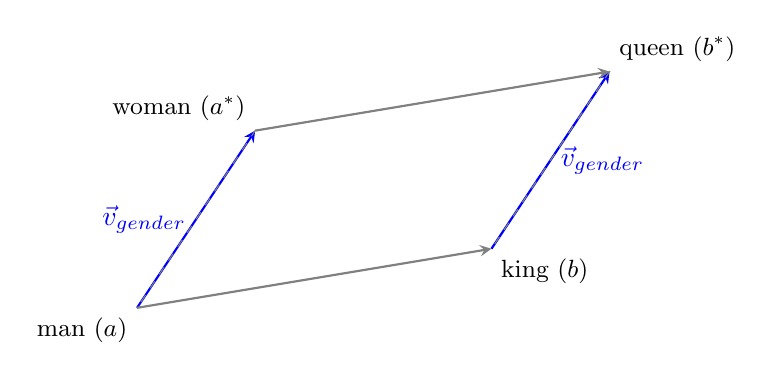
\begin{tikzpicture}[scale=1.5, >=stealth]
    % Coordinate dei punti
    \coordinate (man) at (0,0);
    \coordinate (woman) at (1,1.5);
    \coordinate (king) at (3,0.5);
    \coordinate (queen) at (4,2);

    % Vettori
    \draw[->, thick, blue] (man) -- (woman) node[midway, left] {$\vec{v}_{gender}$};
    \draw[->, thick, blue] (king) -- (queen) node[midway, right] {$\vec{v}_{gender}$};
    \draw[->, thick, gray] (man) -- (king) node[midway, below] {};
    \draw[->, thick, gray] (woman) -- (queen) node[midway, above] {};

    % Nodi (testo)
    \node[below left] at (man) {\small man ($a$)};
    \node[above left] at (woman) {\small woman ($a^*$)};
    \node[below right] at (king) {\small king ($b$)};
    \node[above right] at (queen) {\small queen ($b^*$)};

    % Linee tratteggiate per il parallelogramma
    \draw[dashed, gray] (man) -- (king) -- (queen) -- (woman) -- cycle;
\end{tikzpicture}
\caption{Rappresentazione geometrica del modello del parallelogramma applicato all'analogia di genere.}
\label{fig:parallelogramma}
\end{figure}



Da un punto di vista puramente geometrico, lo spazio degli embeddings è caratterizzato da proprietà di \textbf{parallelismo} e \textbf{ortogonalità}: mentre vettori paralleli indicano relazioni analoghe che si ripetono tra coppie diverse di parole, l’ortogonalità segnala l’indipendenza concettuale tra i termini. In sintesi, queste rappresentazioni apprese in modalità \textit{self-supervised} incorporano automaticamente una vasta gamma di informazioni sintattiche e semantiche, rendendo la scelta della dimensione del vettore e dell’ampiezza della finestra i parametri critici per determinare la qualità del risultato finale. Tuttavia, nonostante la loro straordinaria efficacia, questi modelli presentano un limite intrinseco dovuto alla loro natura \textbf{statica}: ogni parola del vocabolario è associata a un unico vettore che deve condensare in sé tutti i possibili sensi del termine, rendendo difficile la gestione della polisemia. Per superare questa rigidità e permettere alla rappresentazione di adattarsi dinamicamente al contesto specifico di ogni singola frase, la ricerca si è evoluta verso lo sviluppo degli \textbf{embeddings dinamici}.


\section{Contextual Embeddings}

Nelle sezioni precedenti abbiamo visto che gli embeddings statici, una volta
completata la fase di addestramento, associano a ciascuna parola del vocabolario una
rappresentazione vettoriale fissa. In questo approccio, il significato di una parola è
modellato come una proprietà stabile e indipendente dal contesto in cui essa appare.
Tuttavia, il significato linguistico non è un’entità immutabile, ma dipende in modo
cruciale dal contesto sintattico e semantico in cui una parola viene utilizzata.

Una stessa parola può infatti esprimere significati diversi (polisemia), come nel
caso di termini quali \textit{spesso}, che può riferirsi sia a una frequenza sia a una
caratteristica di spessore. Inoltre, anche quando il senso rimane invariato, il
contributo semantico di una parola può variare in profondità e sfumature a seconda
della frase in cui compare. Queste osservazioni rendono evidente il limite degli
embeddings statici e motivano la necessità di rappresentazioni del significato
capaci di adattarsi dinamicamente al contesto.

Per rispondere a questa esigenza sono stati introdotti i \textit{contextual
embeddings}, ovvero rappresentazioni vettoriali che modellano il significato di una
parola come funzione dell’intera sequenza in cui essa appare. A differenza degli
embeddings statici, gli embeddings contestuali non sono parametri direttamente
associati alle parole del vocabolario, ma emergono come risultato dell’elaborazione
di una sequenza di testo da parte di un modello di linguaggio neurale.

\medskip

\noindent
Dato un modello di linguaggio pre--addestrato e una nuova frase in input, è possibile
interpretare la sequenza dei vettori di uscita del modello come un insieme di
embeddings contestuali, uno per ciascun token della frase. Tali vettori catturano
informazioni sintattiche e semantiche dipendenti dal contesto e possono essere
utilizzati in qualsiasi task che richieda una rappresentazione del significato di
parole o token in contesto.

\begin{notebox}
\textbf{Embeddings contestuali}\\
Data una sequenza di token di input $x_1, \ldots, x_n$, un modello di linguaggio
produce una sequenza di vettori di uscita $h_1^{(L)}, \ldots, h_n^{(L)}$, dove $L$
denota l’ultimo strato del modello. Il vettore $h_i^{(L)}$ rappresenta il significato
del token $x_i$ nel contesto della sequenza $x_1, \ldots, x_n$.
\end{notebox}

\noindent
Nella pratica, anziché utilizzare esclusivamente il vettore di uscita dell’ultimo
strato del modello, è comune costruire la rappresentazione contestuale di un token
combinando le informazioni provenienti da più livelli. Una scelta frequente consiste
nel calcolare la media dei vettori di uscita degli ultimi quattro strati,
ovvero $h_i^{(L)}, h_i^{(L-1)}, h_i^{(L-2)}$ e $h_i^{(L-3)}$, ottenendo una
rappresentazione più robusta che integra informazioni a diversi livelli di
astrazione.

\medskip

\noindent
Questa distinzione è concettualmente fondamentale: mentre gli embeddings statici
rappresentano il significato di \emph{tipi di parola} (word types), gli embeddings
contestuali rappresentano il significato di \emph{istanze di parola} (word
instances), ovvero di una parola specifica all’interno di un contesto specifico.
In altre parole, il significato non è più una proprietà intrinseca della parola, ma il
risultato della sua interazione con le altre parole della sequenza.

\medskip

\noindent
Per comprendere come tali rappresentazioni contestuali vengano effettivamente
generate, è ora necessario analizzare il funzionamento dei modelli di linguaggio
neurali, che costituiscono la sorgente primaria degli embeddings contestuali.




\section{Modelli di linguaggio neurali}
\label{sec:neural_language_models}

I \textit{modelli di linguaggio neurali} costituiscono il meccanismo fondamentale
attraverso cui vengono generate le rappresentazioni contestuali introdotte nella
sezione precedente. L’idea centrale è che, per poter predire correttamente una
parola in un determinato contesto, un modello debba necessariamente costruire una
rappresentazione interna del contesto stesso. È proprio questa rappresentazione
interna che, nei modelli moderni, viene interpretata come embedding contestuale.

\begin{notebox}
Formalmente, un modello di linguaggio assegna una probabilità a una sequenza di
token $x_1, \ldots, x_n$. Nei modelli neurali tale probabilità viene fattorizzata
tramite la regola della catena:
\[
P(x_1, \ldots, x_n) = \prod_{i=1}^{n} P(x_i \mid x_1, \ldots, x_{i-1}),
\]
riducendo il problema alla stima della probabilità della parola successiva dato il
contesto precedente. Il compito del modello è quindi quello di apprendere le
regolarità statistiche, sintattiche e semantiche del linguaggio a partire da grandi
corpora testuali.
\end{notebox}



Durante l’inferenza forward (o \textit{decoding}), dato un contesto di parole
precedenti, il modello esegue un forward pass sulla rete neurale per produrre una
distribuzione di probabilità sulle possibili parole successive. Nei primi modelli di
linguaggio neurali, il contesto osservabile è limitato a una finestra di dimensione
fissa che considera un numero $N$ di parole nel passato. Per chiarezza espositiva,
consideriamo il caso $N = 3$, in cui il contesto è costituito dalle parole
$w_{t-1}$, $w_{t-2}$ e $w_{t-3}$. Ciascuna parola del contesto viene inizialmente rappresentata come un vettore
\textit{one-hot} di dimensione $|V|$, dove $|V|$ è la dimensione del vocabolario.
Questi vettori vengono poi proiettati in uno spazio denso tramite una matrice di
embedding $E \in \mathbb{R}^{d \times |V|}$. La moltiplicazione della matrice $E$
per un vettore one-hot seleziona la colonna corrispondente alla parola, producendo il
suo embedding vettoriale. Gli embedding delle parole di contesto vengono quindi
concatenati per formare un unico vettore di input $e$.

\medskip

\noindent
Il vettore $e$ viene successivamente trasformato da uno strato nascosto della rete,
tramite una moltiplicazione per una matrice di pesi $W$, l’aggiunta di un termine di
bias $b$ e l’applicazione di una funzione di attivazione non lineare $\sigma$,
ottenendo lo stato nascosto $h$. Lo stato nascosto viene quindi proiettato nello
spazio delle dimensioni del vocabolario tramite una seconda matrice di pesi $U$,
generando un vettore di punteggi $z$. L’ultimo passo consiste nell’applicazione della funzione \textit{softmax}, che
trasforma i punteggi in una distribuzione di probabilità. Dopo l’applicazione del
softmax, ciascun nodo $i$ dello strato di uscita stima la probabilità che la parola
successiva $w_t$ sia la parola del vocabolario con indice $i$, dato il contesto:
\[
P(w_t = i \mid w_{t-1}, w_{t-2}, w_{t-3}).
\]
In sintesi, le equazioni di un modello di linguaggio neurale feedforward con finestra
di contesto di dimensione 3, dati vettori di input one-hot per ciascuna parola di
contesto, sono le seguenti:
\begin{equation}
\begin{aligned}
e &= [E x_{t-3};\ E x_{t-2};\ E x_{t-1}] \\
h &= \sigma(W e + b) \\
z &= U h \\
\hat{y} &= \text{softmax}(z)
\end{aligned}
\tag{3.1}
\end{equation}

\noindent
Si noti che il vettore di embedding $e$ è ottenuto concatenando gli embedding delle
parole di contesto; nel seguito utilizzeremo il punto e virgola per indicare la
concatenazione di vettori. Sebbene questi modelli siano in grado di apprendere rappresentazioni
distribuzionali utili e abbiano rappresentato un passo fondamentale verso la
modellazione neurale del linguaggio, essi presentano limiti strutturali evidenti. In
particolare, la dimensione del contesto è fissa e l’informazione contestuale viene
compressa in un’unica rappresentazione, rendendo difficile catturare dipendenze a
lungo raggio e strutture sintattiche complesse. Questi limiti hanno motivato lo sviluppo di modelli sequenziali più espressivi, in
grado di aggiornare dinamicamente la rappresentazione del contesto man mano che
la sequenza viene processata. Nel prossimo paragrafo analizzeremo le
\textit{Recurrent Neural Networks} (RNN) e le loro estensioni, le
\textit{Long Short-Term Memory} (LSTM), che rappresentano il primo tentativo
sistematico di modellare il linguaggio come una sequenza di lunghezza variabile e di
produrre embeddings contestuali dipendenti dall’intera storia precedente.


\section{Reti neurali ricorrenti e LSTM}
\label{sec:rnn_lstm}

I modelli di linguaggio neurali feedforward introdotti nella sezione precedente
rappresentano un primo passo verso la modellazione distribuzionale del linguaggio,
ma soffrono di un limite strutturale fondamentale: il contesto è limitato a una
finestra di dimensione fissa e non può adattarsi dinamicamente alla lunghezza della
sequenza. Per superare questo vincolo, sono state introdotte le
\textit{Recurrent Neural Networks} (RNN), architetture progettate per elaborare
sequenze di lunghezza arbitraria mantenendo una rappresentazione del contesto che
viene aggiornata passo dopo passo.

\medskip

\noindent
In una RNN, la sequenza di input viene processata iterativamente. A ogni passo
temporale $t$, il modello riceve in input il token corrente $x_t$ e aggiorna uno
\textit{stato nascosto} $h_t$, che dipende sia dall’input corrente sia dallo stato
precedente:
\[
h_t = f(h_{t-1}, x_t),
\]
dove $f$ è una funzione non lineare parametrizzata. Lo stato nascosto $h_t$
costituisce una rappresentazione compatta del contesto osservato fino al passo $t$ e
può essere interpretato come una rappresentazione contestuale del token corrente.

\medskip

\noindent
Nei modelli di linguaggio basati su RNN, la probabilità della parola successiva viene
stimata a partire dallo stato nascosto corrente:
\[
P(w_t \mid w_1, \ldots, w_{t-1}) = g(h_{t-1}),
\]
dove $g$ è tipicamente una trasformazione affine seguita da una funzione softmax.
In questo modo, la RNN è in grado di modellare dipendenze sequenziali senza imporre
un limite fisso alla dimensione del contesto, rappresentando un avanzamento
significativo rispetto ai modelli feedforward.

\medskip

\noindent
Nonostante questi vantaggi, le RNN presentano importanti difficoltà nell’apprendere
dipendenze a lungo raggio. Durante l’addestramento tramite backpropagation through
time, i gradienti possono tendere a svanire o esplodere, rendendo difficile
l’aggiornamento efficace dei parametri per sequenze lunghe. Questo problema,
noto come \textit{vanishing gradient problem}, limita la capacità delle RNN di
catturare relazioni distanti nel testo.

\medskip

\noindent
Per affrontare tali limiti sono state introdotte le \textit{Long Short-Term Memory}
(LSTM), una variante delle RNN progettata per mantenere e aggiornare informazioni
rilevanti su orizzonti temporali più lunghi. Le LSTM introducono una struttura di
memoria esplicita, controllata da meccanismi di gating, che regolano quali
informazioni debbano essere conservate, aggiornate o dimenticate nel tempo. Grazie
a questi meccanismi, le LSTM risultano più stabili durante l’addestramento e più
efficaci nel modellare dipendenze a lungo raggio.

\medskip

\noindent
Dal punto di vista delle rappresentazioni, gli stati nascosti prodotti da RNN e LSTM
possono essere interpretati come le prime forme di \emph{embeddings contestuali}
appresi da modelli di linguaggio neurali. Ogni token è associato a un vettore che
dipende dall’intera storia precedente della sequenza, consentendo di distinguere
occorrenze diverse della stessa parola in contesti diversi.

\medskip

\noindent
Tuttavia, anche le LSTM presentano limiti strutturali rilevanti. In primo luogo, il
contesto viene comunque compresso in un singolo stato nascosto, che deve riassumere
tutta l’informazione rilevante della sequenza precedente. In secondo luogo, le RNN e
le LSTM elaborano la sequenza in modo intrinsecamente sequenziale, impedendo una
parallelizzazione efficiente del calcolo. Infine, nei modelli di linguaggio standard,
il contesto utilizzato è tipicamente unidirezionale, limitato alle parole precedenti.

\medskip

\noindent
Questi limiti hanno motivato lo sviluppo di modelli in grado di sfruttare informazioni
provenienti sia dal contesto sinistro sia da quello destro di una parola. Nel
prossimo paragrafo analizzeremo ELMo, un modello che introduce embeddings
contestuali bidirezionali basati su reti ricorrenti, rappresentando un’importante
tappa intermedia nel percorso che conduce ai modelli basati sull’architettura
Transformer.


\section{ELMo e il contesto bidirezionale}
\label{sec:elmo}

Le RNN e le LSTM introducono per la prima volta rappresentazioni contestuali
dipendenti dalla sequenza, ma nei modelli di linguaggio standard tali
rappresentazioni sono tipicamente \emph{unidirezionali}, poiché il contesto utilizzato
per predire una parola è limitato alle parole precedenti. Tuttavia, molti compiti di
comprensione del linguaggio naturale richiedono di interpretare una parola alla luce
dell’intera frase, includendo anche il contesto destro. Questa osservazione ha
motivato lo sviluppo di modelli in grado di produrre rappresentazioni
contestuali \emph{bidirezionali}.

\medskip

\noindent
ELMo (\textit{Embeddings from Language Models}) rappresenta uno dei primi modelli
in grado di fornire embeddings contestuali profondi e bidirezionali. Il modello è
basato su una architettura \textit{biLSTM}, ovvero due LSTM separate che processano
la sequenza in direzione sinistra--destra e destra--sinistra. Le rappresentazioni
prodotte da entrambe le direzioni vengono quindi combinate per ottenere un embedding
contestuale per ciascun token.

\medskip

\noindent
Un aspetto distintivo di ELMo è l’utilizzo di rappresentazioni \emph{stratificate}. Il
modello produce infatti più livelli di rappresentazione per ogni token, ciascuno dei
quali cattura informazioni linguistiche a diversi livelli di astrazione. Le
rappresentazioni finali utilizzate nei task downstream non corrispondono
necessariamente all’output di un singolo strato, ma vengono ottenute come
combinazione pesata degli stati prodotti dai diversi strati del modello.

\medskip

\noindent
Dal punto di vista semantico, ELMo fornisce embeddings distinti per ogni occorrenza
di una parola, consentendo di catturare in modo efficace fenomeni di polisemia e
disambiguazione del senso. In questo senso, ELMo rappresenta un passaggio cruciale
nel superamento definitivo del paradigma degli embeddings statici e dimostra
empiricamente l’utilità delle rappresentazioni contestuali profonde per una vasta
gamma di compiti linguistici.

\medskip

\noindent
Nonostante questi progressi, ELMo eredita alcuni limiti strutturali dalle architetture
ricorrenti su cui è basato. In particolare, l’elaborazione della sequenza rimane
intrinsecamente sequenziale, limitando la possibilità di parallelizzazione del
calcolo. Inoltre, sebbene la bidirezionalità consenta di sfruttare l’intero contesto,
l’informazione deve comunque essere mediata attraverso stati ricorrenti, rendendo
difficile modellare direttamente dipendenze molto distanti nella sequenza.

\medskip

\noindent
Questi limiti hanno motivato l’introduzione di un nuovo paradigma architetturale, in
cui le parole di una sequenza possono interagire direttamente tra loro senza essere
mediate da uno stato ricorrente. Nel prossimo paragrafo introdurremo il meccanismo
di \textit{attention} e, in particolare, la \textit{self-attention}, che costituisce il
fondamento dei modelli Transformer.


\section{Attention e Self-Attention}
\label{sec:attention}

I modelli basati su RNN e LSTM, inclusi quelli bidirezionali come ELMo, producono
rappresentazioni contestuali efficaci, ma presentano un limite strutturale comune:
l’informazione contestuale deve essere mediata attraverso uno stato ricorrente che
riassume l’intera sequenza. Questo meccanismo di compressione rende difficile
modellare in modo diretto dipendenze a lungo raggio e relazioni complesse tra parole
distanti nella frase.

\medskip

\noindent
Per superare questo limite è stato introdotto il meccanismo di \textit{attention}, che
permette a un modello di selezionare dinamicamente le parti più rilevanti del
contesto quando deve produrre una rappresentazione o una predizione. L’idea
fondamentale dell’attention è che, anziché affidarsi a una singola rappresentazione
globale del contesto, il modello possa accedere direttamente a tutte le
rappresentazioni disponibili e assegnare loro un peso in base alla rilevanza rispetto
a un determinato obiettivo.

\medskip

\noindent
In termini intuitivi, il meccanismo di attention consente al modello di rispondere
alla domanda: \emph{quali parole del contesto sono più informative per interpretare
il token corrente?} I pesi di attenzione determinano l’importanza relativa di ciascun
token del contesto e vengono utilizzati per combinare le rappresentazioni disponibili
in una nuova rappresentazione contestuale.

\medskip

\noindent
Un’evoluzione fondamentale di questo meccanismo è rappresentata dalla
\textit{self-attention}. A differenza dell’attention classica, in cui l’attenzione è
calcolata tra due sequenze distinte (ad esempio una sequenza sorgente e una
sequenza target), nella self-attention ciascun token di una sequenza può
attendere direttamente a tutti gli altri token della stessa sequenza. In questo modo,
ogni parola costruisce la propria rappresentazione contestuale come combinazione
pesata delle rappresentazioni di tutte le altre parole della frase.

\medskip

\noindent
La self-attention presenta diversi vantaggi rispetto ai modelli ricorrenti. In primo
luogo, consente di modellare direttamente dipendenze a lungo raggio, poiché la
distanza tra due token nella sequenza non influisce sulla loro capacità di interagire.
In secondo luogo, l’elaborazione della sequenza non è più intrinsecamente
sequenziale: le rappresentazioni di tutti i token possono essere calcolate in
parallelo, migliorando significativamente l’efficienza computazionale e la
scalabilità del modello.

\medskip

\noindent
Dal punto di vista delle rappresentazioni, la self-attention produce per ciascun
token una rappresentazione contestuale che integra informazioni provenienti
dall’intera sequenza. Il significato di una parola emerge quindi come risultato
esplicito delle interazioni con tutte le altre parole della frase, piuttosto che come
un riassunto implicito codificato in uno stato ricorrente.

\medskip

\noindent
Tuttavia, il meccanismo di attention da solo non definisce un modello completo di
linguaggio o di rappresentazione. Per ottenere un’architettura in grado di produrre
rappresentazioni contestuali profonde e composizionali è necessario combinare la
self-attention con ulteriori componenti strutturali, come trasformazioni non lineari,
meccanismi di normalizzazione e informazioni sulla posizione dei token nella
sequenza.

\medskip

\noindent
Nel prossimo paragrafo introdurremo l’architettura Transformer, che integra il
meccanismo di self-attention in una struttura modulare e profonda, costituendo il
fondamento dei moderni modelli di linguaggio basati su embeddings contestuali,
incluso BERT.



\section{BERT e Masked Language Modeling}
\label{sec:bert}

L’architettura Transformer encoder introdotta nella sezione precedente fornisce un
meccanismo potente per la costruzione di rappresentazioni contestuali, ma da sola
non determina come tali rappresentazioni debbano essere apprese né quale obiettivo
di addestramento sia più adatto ai compiti di comprensione del linguaggio naturale.
BERT (\textit{Bidirectional Encoder Representations from Transformers}) rappresenta
una risposta a questa esigenza, combinando il Transformer encoder con un obiettivo
di addestramento specificamente progettato per produrre embeddings contestuali
profondamente bidirezionali.

\medskip

\noindent
A differenza dei modelli di linguaggio causali, che predicono la parola successiva
utilizzando esclusivamente il contesto sinistro, BERT utilizza un Transformer
\emph{encoder-only} e adotta un obiettivo di addestramento che consente al modello di
sfruttare simultaneamente il contesto sinistro e destro di ciascun token. Questa
caratteristica rende BERT particolarmente adatto a compiti interpretativi, come la
classificazione di testo, il riconoscimento di entità nominate e la disambiguazione
del senso delle parole.

\medskip

\noindent
Il principale obiettivo di addestramento di BERT è il \textit{Masked Language
Modeling} (MLM). Durante il pretraining, una frazione dei token di una frase viene
mascherata e il modello è addestrato a predire i token originali a partire dal contesto
circostante. In questo modo, il modello è costretto a costruire rappresentazioni che
integrano informazioni provenienti da entrambe le direzioni della sequenza, dando
luogo a embeddings contestuali profondamente bidirezionali.

\medskip

\noindent
Dal punto di vista architetturale, l’input di BERT è costituito dalla somma di tre
componenti: l’embedding del token (tipicamente ottenuto tramite una
tokenizzazione a sotto-parole), l’embedding di posizione e un embedding di segmento
utilizzato per distinguere parti diverse dell’input. L’output del modello è una
sequenza di vettori contestuali, uno per ciascun token, prodotti dall’ultimo strato
del Transformer encoder.

\medskip

\noindent
Un elemento distintivo di BERT è l’introduzione di un token speciale \texttt{[CLS]},
inserito all’inizio della sequenza di input. Il vettore contestuale associato a questo
token viene spesso utilizzato come rappresentazione dell’intera sequenza in compiti
di classificazione. Parallelamente, i vettori associati agli altri token forniscono
rappresentazioni contestuali a livello di parola, utilizzabili per compiti di
annotazione sequenziale e analisi semantica.

\medskip

\noindent
Come nei modelli contestuali precedenti, anche in BERT è comune non utilizzare
esclusivamente il vettore di uscita dell’ultimo strato, ma combinare le
rappresentazioni provenienti da più livelli del modello. In particolare, la media o
la somma dei vettori degli ultimi strati consente di integrare informazioni a diversi
livelli di astrazione, rendendo gli embeddings più robusti e informativi.

\medskip

\noindent
Il paradigma di addestramento di BERT segue lo schema \textit{pretrain}--\textit{finetune}.
Nella fase di pretraining, il modello apprende rappresentazioni generali del
linguaggio a partire da grandi quantità di testo non annotato. Nella fase di
finetuning, tali rappresentazioni vengono adattate a specifici compiti downstream
mediante l’aggiunta di teste di classificazione leggere e un addestramento
supervisionato su dataset più piccoli.

\medskip

\noindent
Dal punto di vista delle rappresentazioni, BERT produce embeddings contestuali
profondi, stratificati e ad alta dimensionalità, che incorporano in modo entangled
informazioni sintattiche, semantiche e pragmatiche. Questa ricchezza rappresentativa
è una delle principali ragioni del successo empirico di BERT, ma rende al contempo
complessa l’interpretazione delle singole dimensioni e delle strutture latenti degli
embedding.

\medskip

\noindent
Nel prossimo paragrafo discuteremo perché tali rappresentazioni, pur essendo
estremamente efficaci, beneficiano di tecniche di analisi e \textit{disentanglement},
motivando l’utilizzo di metodi basati su autoencoder sparsi per l’interpretazione e la
scomposizione degli embeddings di BERT, che costituisce l’obiettivo principale di
questa tesi.

\section{Motivazione per il disentanglement degli embeddings di BERT}
\label{sec:motivation_disentanglement}

Il percorso seguito in questo capitolo ha mostrato come gli embeddings moderni,
in particolare quelli prodotti da BERT, rappresentino il punto di arrivo di una
progressiva evoluzione delle rappresentazioni distribuzionali del linguaggio: da
vettori statici associati a tipi di parola a rappresentazioni contestuali profonde,
dipendenti dall’intera sequenza e apprese tramite modelli di linguaggio neurali
bidirezionali.

\medskip

\noindent
Gli embeddings di BERT sono caratterizzati da un’elevata capacità rappresentativa.
Essi catturano simultaneamente informazioni sintattiche, semantiche e pragmatiche,
distribuite su molte dimensioni e stratificate lungo i diversi livelli del modello.
Questa ricchezza informativa è alla base delle eccellenti prestazioni empiriche di
BERT in una vasta gamma di compiti di elaborazione del linguaggio naturale.

\medskip

\noindent
Tuttavia, tale potenza rappresentativa ha un costo in termini di interpretabilità.
Le informazioni codificate negli embeddings di BERT risultano fortemente
\emph{entangled}: singole dimensioni non corrispondono a proprietà linguistiche
chiaramente interpretabili e le strutture latenti che emergono nello spazio
vettoriale sono difficili da analizzare direttamente. Di conseguenza, comprendere
quali fattori semantici o sintattici contribuiscano a una determinata rappresentazione
diventa un compito non banale.

\medskip

\noindent
Questo problema è particolarmente rilevante nel contesto di applicazioni che
richiedono trasparenza, analisi qualitativa o controllo delle rappresentazioni
interne del modello. In tali scenari, non è sufficiente disporre di embeddings
accurati: è necessario poterli interpretare, analizzare e, in alcuni casi,
scomporre in componenti latenti più semplici e semanticamente coerenti.

\medskip

\noindent
Le tecniche di \textit{disentanglement} delle rappresentazioni mirano proprio a
questo obiettivo: separare i fattori latenti che contribuiscono alla costruzione di
una rappresentazione densa, rendendo esplicite strutture che risultano altrimenti
sovrapposte. In questo contesto, gli autoencoder sparsi rappresentano uno strumento
particolarmente adatto, poiché consentono di apprendere rappresentazioni latenti
compatte in cui solo un numero limitato di componenti è attivo per ciascun input.

\medskip

\noindent
Applicare tecniche di disentanglement agli embeddings di BERT consente quindi di
analizzare la struttura interna di queste rappresentazioni, individuare dimensioni o
fattori latenti interpretabili e studiare come diverse proprietà linguistiche
emergano nello spazio vettoriale. Questo approccio permette di coniugare l’elevata
capacità rappresentativa dei modelli di linguaggio moderni con un maggiore grado di
interpretabilità.

\medskip

\noindent
Nel capitolo successivo introdurremo il formalismo degli autoencoder e, in
particolare, degli \textit{sparse autoencoders}, discutendone le proprietà teoriche
e il loro utilizzo come strumento per il disentanglement di rappresentazioni dense.
Successivamente, tali tecniche verranno applicate agli embeddings di BERT
attraverso l’applicazione sviluppata in questa tesi, fornendo un caso di studio
concreto sull’analisi e l’interpretazione delle rappresentazioni contestuali.


\section{Pooling}

Data una sequenza di token
\begin{equation*}
(t_1, \dots, t_N),
\end{equation*}
ottenuta dalla tokenizzazione di un testo e fornita in input a un modello
Transformer di tipo BERT-like, il modello non restituisce una singola
rappresentazione vettoriale dell’intera sequenza, bensì una sequenza di
rappresentazioni contestuali a livello di token. Più precisamente, l’output
del modello può essere espresso come una matrice
\begin{equation*}
\mathbf{H} =
\begin{bmatrix}
\mathbf{h}_1 \\
\mathbf{h}_2 \\
\vdots \\
\mathbf{h}_N
\end{bmatrix}
\in \mathbb{R}^{N \times d},
\end{equation*}
dove $d$ indica la dimensionalità dello spazio latente del modello e ciascun
vettore $\mathbf{h}_i \in \mathbb{R}^{d}$ rappresenta l’embedding contestuale
del token $t_i$, ovvero una codifica che incorpora informazione proveniente
dall’intera sequenza grazie al meccanismo di self-attention.
In molte applicazioni di elaborazione del linguaggio naturale, tuttavia, non
si è interessati a una rappresentazione a livello di singolo token, bensì a un
unico vettore che riassuma il significato complessivo dell’intera sequenza,
come nel caso della similarità semantica, del clustering di testi o della
classificazione a livello di frase o documento. Per ottenere tale
rappresentazione globale è quindi necessario introdurre un’operazione di
\textit{pooling}.

Formalmente, un’operazione di pooling è una funzione che aggrega una
collezione di vettori in un singolo vettore:
\begin{equation*}
\text{Pooling} : \mathbb{R}^{N \times d} \rightarrow \mathbb{R}^{d}.
\end{equation*}
Applicando tale funzione alla matrice di embedding token-level $\mathbf{H}$,
si ottiene un vettore
\begin{equation*}
\mathbf{v} = \text{Pooling}(\mathbf{H}),
\end{equation*}
che può essere interpretato come una rappresentazione vettoriale globale
della sequenza di input, intesa come unità semantica.
L’operazione di pooling realizza dunque una riduzione strutturale lungo la
dimensione dei token, trasformando una rappresentazione distribuita su $N$
elementi in un singolo punto nello spazio latente. La scelta della funzione di
pooling non è univoca e dipende sia dal modello utilizzato sia dal tipo di
informazione che si desidera preservare.

\subsubsection{Strategie di pooling}

Le principali strategie di pooling utilizzate per ottenere una
rappresentazione vettoriale globale a partire dalle rappresentazioni
token-level prodotte da modelli Transformer possono essere descritte come
segue.

\begin{itemize}

\item \textbf{Mean pooling}.  
Una delle strategie più semplici e diffuse consiste nel calcolare la media
aritmetica dei vettori associati ai singoli token:
\begin{equation*}
\mathbf{v} = \frac{1}{N} \sum_{i=1}^{N} \mathbf{h}_i.
\end{equation*}
Questa operazione assegna a ciascun token lo stesso peso e produce una
rappresentazione che riflette il contributo medio dell’intera sequenza.
Il mean pooling è particolarmente adatto a compiti di similarità semantica
e ad analisi distribuzionali del significato, poiché preserva l’informazione
globale senza privilegiare posizioni specifiche della sequenza.

\item \textbf{Max pooling}.  
Un’alternativa è rappresentata dal max pooling, in cui ciascuna componente
del vettore finale è ottenuta selezionando il valore massimo osservato tra
tutti i token:
\begin{equation*}
\mathbf{v}_j = \max_{i=1,\dots,N} (\mathbf{h}_{i,j}),
\end{equation*}
dove $\mathbf{h}_{i,j}$ indica la $j$-esima componente del vettore
$\mathbf{h}_i$. Questa strategia enfatizza le feature più salienti presenti
nella sequenza, catturando segnali forti anche se localizzati in un numero
limitato di token, ma tende a sacrificare l’informazione distribuita lungo
l’intero testo.

\item \textbf{Token speciale di classificazione (\texttt{[CLS]})}.  
Nei modelli BERT-like è comune utilizzare il vettore associato a un token
speciale, tipicamente \texttt{[CLS]}, come rappresentazione globale della
sequenza:
\begin{equation*}
\mathbf{v} = \mathbf{h}_{\texttt{[CLS]}}.
\end{equation*}
In questo caso, il pooling non consiste in un’aggregazione esplicita dei
vettori token-level, ma nella selezione di un singolo vettore. Il token
\texttt{[CLS]} viene infatti addestrato durante il pretraining del modello
a catturare informazione a livello di sequenza, svolgendo il ruolo di una
rappresentazione globale implicita, particolarmente adatta a task di
classificazione.

\item \textbf{Pooling appreso}.  
Una classe più generale di approcci consiste nell’apprendere
l’operazione di pooling tramite un modello parametrico. In questo caso,
la rappresentazione globale è ottenuta applicando una funzione
$P_{\theta}$, tipicamente implementata come una rete neurale, alla matrice
delle rappresentazioni token-level:
\begin{equation*}
\mathbf{v} = P_{\theta}(\mathbf{H}).
\end{equation*}
Questo approccio consente di assegnare pesi differenti ai token e di
modellare interazioni più complesse rispetto alle strategie statiche,
al costo di una maggiore complessità del modello e della necessità di
obiettivi di addestramento specifici.

\end{itemize}

Alcune famiglie di modelli, come i \textit{Sentence-Transformers},
integrano direttamente l’operazione di pooling all’interno
dell’architettura. In tali modelli, un backbone Transformer produce le
rappresentazioni token-level, che vengono immediatamente aggregate tramite
una delle strategie descritte (tipicamente mean pooling), e l’intero
sistema è addestrato end-to-end per produrre embedding a livello di frase
ottimizzati per compiti di similarità semantica e retrieval.

\subsection{Pooling gerarchico per sequenze lunghe}

I modelli Transformer di tipo BERT-like impongono un vincolo strutturale
sulla lunghezza massima della sequenza di input, tipicamente indicata con
$L_{\max}$. Quando una sequenza di token supera tale limite, non è possibile
processarla integralmente in un singolo forward pass del modello. Sia quindi
dato un testo tokenizzato come
\begin{equation*}
T = (t_1, \dots, t_N),
\end{equation*}
con $N > L_{\max}$. In questo caso, per ottenere una rappresentazione
vettoriale globale del testo senza ricorrere alla troncatura, è necessario
adottare una strategia di aggregazione su più livelli.

\paragraph{Segmentazione in chunk}
La sequenza $T$ viene suddivisa in $K$ sotto-sequenze contigue (chunk)
\begin{equation*}
C_1, C_2, \dots, C_K,
\end{equation*}
ciascuna di lunghezza al più $W_{\text{eff}} \le L_{\max}$, dove
$W_{\text{eff}}$ rappresenta la lunghezza massima effettivamente disponibile
per i token di contenuto, una volta considerati eventuali token speciali
richiesti dal modello. Formalmente,
\begin{equation*}
C_k = (t_{(k-1)W_{\text{eff}}+1}, \dots, t_{\min(kW_{\text{eff}},\,N)}),
\qquad k = 1, \dots, K.
\end{equation*}

\paragraph{Pooling a livello di token (intra-chunk)}
Ciascun chunk $C_k$ viene processato indipendentemente dal modello
Transformer, che produce una matrice di rappresentazioni token-level
\begin{equation*}
\mathbf{H}^{(k)} \in \mathbb{R}^{m_k \times d},
\end{equation*}
dove $m_k$ è il numero di token del chunk $k$ e $d$ è la dimensionalità
latente del modello. Applicando una funzione di pooling a livello di token,
si ottiene un embedding rappresentativo del singolo chunk:
\begin{equation*}
\mathbf{e}_k = \text{Pooling}_{\text{token}}\!\left(\mathbf{H}^{(k)}\right),
\qquad \mathbf{e}_k \in \mathbb{R}^{d}.
\end{equation*}
Questa prima operazione di pooling realizza una riduzione dalla
rappresentazione distribuita sui token a una rappresentazione compatta a
livello di segmento.

\paragraph{Pooling a livello di chunk (inter-chunk)}
Una volta ottenuti gli embedding dei singoli chunk
$\mathbf{e}_1, \dots, \mathbf{e}_K$, è necessario aggregarli per costruire
una rappresentazione globale dell’intero testo. Tale aggregazione può essere
formalizzata come una seconda operazione di pooling:
\begin{equation*}
\mathbf{v}_D = \text{Pooling}_{\text{chunk}}
\bigl(\mathbf{e}_1, \dots, \mathbf{e}_K\bigr),
\qquad \mathbf{v}_D \in \mathbb{R}^{d}.
\end{equation*}
Nel caso più semplice, adottato in questo lavoro, la funzione
$\text{Pooling}_{\text{chunk}}$ coincide con la media aritmetica:
\begin{equation*}
\mathbf{v}_D = \frac{1}{K} \sum_{k=1}^{K} \mathbf{e}_k.
\end{equation*}

\paragraph{Interpretazione come pooling gerarchico}
La procedura descritta può essere interpretata come una forma di
\textit{pooling gerarchico}. Il primo livello di pooling aggrega
l’informazione a livello di token all’interno di ciascun chunk, mentre il
secondo livello aggrega l’informazione a livello di chunk sull’intero
documento. In questo modo, è possibile ottenere una rappresentazione
vettoriale globale anche per testi di lunghezza arbitraria, preservando il
contributo semantico di tutte le parti della sequenza e mantenendo la
compatibilità con i vincoli architetturali del modello di embedding.
